\documentclass[11pt]{article}


\usepackage{caption}

\usepackage{kotex}
\usepackage{sectsty}
\usepackage{graphicx}
\usepackage{amsmath}
\usepackage[margin=20mm]{geometry}
\usepackage{listings}
\usepackage{color}
\usepackage{lmodern} % Use a slightly nicer looking font
\usepackage{url} % Proper formatting for URLs
\usepackage{graphicx} % Handle inclusion of non-PDF graphics
\usepackage{subfig} % Allow sub-figures inside a figurexz
\usepackage{enumitem} % Allow lists to pick up numbering where the last list left off
\usepackage[margin=20mm]{geometry}
\usepackage{listings}
\usepackage{color}

\usepackage{setspace}
\usepackage{indentfirst}\setlength\parindent{2em}
\setstretch{1.5} %간격 맞추는 패키지


% Color definitions for source code listings
\definecolor{mygreen}{rgb}{0,0.6,0}
\definecolor{mygray}{rgb}{0.5,0.5,0.5}
\definecolor{mymauve}{rgb}{0.58,0,0.82}

\lstset{ 
  backgroundcolor=\color{white},   % choose the background color; you must add \usepackage{color} or \usepackage{xcolor}
  basicstyle=\footnotesize,        % the size of the fonts that are used for the code
  breakatwhitespace=false,         % sets if automatic breaks should only happen at whitespace
  breaklines=true,                 % sets automatic line breaking
  captionpos=b,                    % sets the caption-position to bottom
  commentstyle=\color{mygreen},    % comment style
  deletekeywords={...},            % if you want to delete keywords from the given language
  escapeinside={\%*}{*)},          % if you want to add LaTeX within your code
  extendedchars=true,              % lets you use non-ASCII characters; for 8-bits encodings only, does not work with UTF-8
  frame=single,	                   % adds a frame around the code
  keepspaces=true,                 % keeps spaces in text, useful for keeping indentation of code (possibly needs columns=flexible)
  keywordstyle=\color{blue},       % keyword style
  otherkeywords={*,...},           % if you want to add more keywords to the set
  numbers=left,                    % where to put the line-numbers; possible values are (none, left, right)
  numbersep=5pt,                   % how far the line-numbers are from the code
  numberstyle=\tiny\color{mygray}, % the style that is used for the line-numbers
  rulecolor=\color{black},         % if not set, the frame-color may be changed on line-breaks within not-black text (e.g. comments (green here))
  showspaces=false,                % show spaces everywhere adding particular underscores; it overrides 'showstringspaces'
  showstringspaces=false,          % underline spaces within strings only
  showtabs=false,                  % show tabs within strings adding particular underscores
  stepnumber=2,                    % the step between two line-numbers. If it's 1, each line will be numbered
  stringstyle=\color{mymauve},     % string literal style
  tabsize=2,	                   % sets default tabsize to 2 spaces
  title=\lstname                   % show the filename of files included with \lstinputlisting; also try caption instead of title
}


% Margins
\topmargin=-0.45in
\evensidemargin=0in
\oddsidemargin=0in
\textwidth=6.5in
\textheight=9.0in
\headsep=0.25in


\title{Integration Of Functions Homework 2}
\author{MinWook Kang}
\date{\today}

\begin{document}
\maketitle
\pagebreak

% Optional TOC
% \tableofcontents
% \pagebreak




%--Paper--
\section{Implement Your Own fixed quad in [-1, 1]}

우리는 앞 부분에서, 해를 추정하는 Root Finding Method를 공부했다. 그리고 이번 챕터에서는 Rimann Sum, Trapezoid Rule, Simpsion's Rule 그리고 Gaussian Quadrature을 통하여 어떤 함수 f 가 주어졌을 때, 우리가 원하는 범위 안에서의 적분 값을 실제의 적분 값과 매우 비슷하게 추정할 수 있는 방법을 배웠다. 이것으로 실제로 적분이 필요한 문제들에 대해 접근해 보겠다.
\subsection{Problem Recognition} 
SciPy 모듈에서 fixed quad를 사용하면, Gaussian Quadrature 의 방식으로 원하는 적분 범위 안에서의 적분 값을 유추할 수 있다. 하지만, 이 모듈을 사용하지 않고, 모듈을 만들어서 문제에 적용하는 것을 보일 것이다. 
\begin{equation}
\int_{-1}^{1} e^x dx = e - e^{-1} \approx 2.3504023872876029138
\end{equation}

$F(x) = e^x$ 를 [-1, 1]로 적분하게 되면 나오는 값을 구하는 모듈을 만들어야 한다. Gauss-Legendre 방식에 의하면, [-1, 1]에서 N에 대한 $x_i$ 값과 $w_i$ 값을 알고 이것을 곱하여 더하게 되면, 

\begin{equation}
\int_{-1}^1 f(x) dx \approx \sum_{i = 1}^n w_i f(x_i) \equiv G_n(f)
\end{equation}

위의 공식에 따라, [-1, 1] 사이의 적분 값을 추산할 수 있다. 따라서 우리는 먼저 $x_i$ 값과 $w_i$ 값을 구해줄 것이다. 그러기 위해서는 우선, 임의의 숫자 N에 대한 르장드르 다항식의 해가 필요한데, 이는  SciPy 모듈에서 roots\textunderscore legendre 을 통해 쉽게 구할 수 있다. 
먼저 roots\textunderscore legendre를 보면, 르장드르 다항식에 들어가는 임의의 숫자 N에 대하여 해 roots 와 무게 weights 값을 알려주는 모듈이다. 만약  N의 값에 3을 대입하면 아래처럼 구할 수 있다.

\begin{lstlisting}[language=Python]
from scipy.special import roots_legendre, eval_legendre
roots, weights = roots_legendre(3)
roots, weights

(array([-0.77459667,  0.        ,  0.77459667]),
 array([0.55555556, 0.88888889, 0.55555556]))
\end{lstlisting}

\subsection{Development of a solution} 
def 함수를 이용하여 min\textunderscore fixed\textunderscore only\textunderscore quad(f, N) 함수를 정의하고, roots 와 weights인수를 xi 와 wi로 저장한 후, zip 함수를 통하여 각 열마다 묶어준 다음, 각각의 $(wi, xi)$ 의 묶음에 따라 식 $w * (f(x))$ 계산한다. 그후 묶음에 대한 이 식들을 더해줌으로서 위의 (2)를 파이썬으로 구현할 것이다. 먼저 $F(x) = e^x$ 이고, 적분 범위는 [-1, 1]이라고 하면 다음과 같다.

\begin{lstlisting}[language=Python]
def f(x):
    return np.exp(x)
    
def min_fixed_only_quad(f, N):
    roots, weights = roots_legendre(N)
    xi = roots
    wi = weights
    return sum(w*(f(x)) for w, x in zip(wi, xi))
print(f"""
n = 1: I  = {min_fixed_only_quad(f, 1)}, Abs error = {(f(1) - f(-1)) - min_fixed_only_quad(f, 1)}
n = 2: I = {min_fixed_only_quad(f, 2)}, Abs error = {(f(1) - f(-1)) - min_fixed_only_quad(f, 2)}
n = 3: I = {min_fixed_only_quad(f, 3)}, Abs error = {(f(1) - f(-1)) - min_fixed_only_quad(f, 3)}
n = 4: I = {min_fixed_only_quad(f, 4)}, Abs error = {(f(1) - f(-1)) - min_fixed_only_quad(f, 4)}
n = 5: I = {min_fixed_only_quad(f, 5)}, Abs error = {(f(1) - f(-1)) - min_fixed_only_quad(f, 5)}
""")

n = 1: I = 2.0, Abs error = 0.35040238728760276
n = 2: I = 2.3426960879097307, Abs error = 0.007706299377872039
n = 3: I = 2.3503369286800115, Abs error = 6.54586075912178e-05
n = 4: I = 2.3504020921563766, Abs error = 2.9513122612456755e-07
n = 5: I = 2.350402386462826, Abs error = 8.247766913882515e-10
\end{lstlisting}

\subsection{Execution and Assessment} 
이때, 우리는 실제 값과의 차이를 비교하기 위하여 $f(1) - f(-1)$ 값에다가 추산한 값을 빼서, N에 따라서 얼만큼 오차가 날 수 있는지 확인해 볼 것이다. 먼저 SciPy package의 fixed\textunderscore quad로 계산한 결과는 다음과 같다.
\begin{lstlisting}[language=Python]
n = 1: approx = (2.0, None)
n = 2: approx = (2.3426960879097307, None)
n = 3: approx = (2.3503369286800115, None)
n = 4: approx = (2.350402092156377, None)
n = 5: approx = (2.350402386462826, None)
\end{lstlisting}

이 두 값을 빼보면, N = 4 인 경우 $-4.440892098500626e-16$ 를 제외하고는 0으로 맞아 떨어지는 것을 볼 수 있다. N=4 인 경우에도, 수가 매우 작으므로, 0이라 봐도 무방하다. 하지만 위의 함수는 범위가 [-1, 1] 로 정해져 있기 때문에, 이를 변수변환을 통해 어느 구간에서도 적분 값을 추산할 수 있는 모듈을 만들 것이다.

\section{Own fixed quad in any range}
\noindent
\subsection{Problem Recognition} 
위의 상황에서는 범위가 [-1, 1]을 만족하는 상황에서만 적분 값을 구할 수 있었다. 그럼 만약, 적분 범위가 아래와 같은 식일 경우는 어떻게 구할 수 있을까? 이는 적분의 범위를 변수변환을 통하여 바꾸어 주면 된다. 

\begin{equation}
\int_0^1 \frac{4}{1 + x^2} dx
\end{equation}


먼저 Gauss' Method에 따르면, $x$ 와 $dx$는 아래처럼 바꾸어도 무방하다.
\begin{equation}
t = \frac{b - a}{2}x + \frac{b + a}{2}
\quad\mathrm{,}\quad
dt = \frac{b - a}{2} dx
\end{equation}

\subsection{Development of a solution} 
 변수 변환을 통해 적분 범위는 $dt$에 대해서 [-1, 1]을 만족하게 된다. 그러면 위의 함수를 조금 변형하면 똑같이 적분을 시킬 수 있다. 위의 def 함수에서, $x$를 $t$에 대한 식으로 바꾸어지고, 함수에 $(b - a) / 2$를 곱하게 해주면 되므로, 위의 식을 $F(x) = \frac{4}{1 + x^2} $ , 적분 범위는 [0, 1]로 잡고 계산하면 다음과 같다.

\begin{lstlisting}[language=Python]
def f(t):
    return np.exp(t)

def min_fixed_any_range(f, a, b, n):
    g = lambda x: (b - a)/2 * f((b-a)/2*x + (a+b)/2) 
    roots, weights = roots_legendre(n)
    xi = roots
    wi = weights
    return sum(w*(g(x)) for w, x in zip(wi, xi))
\end{lstlisting}

먼저 def로 선언한 함수를 보면 인수를 4개로 두었는데, 이는 구하고자 하는 함수의 범위를 나타내며, 변수 변환을 통해 원하는 [a, b] 의 적분 값을 구할 수 있다. 또한 $g(x)$ 라는 함수에 대해 lambda를 통하여 아래의 식을 새롭게 정의 하였다.
\begin{equation}
g(x) = \frac{b - a}{2}  f( \frac{b - a}{2}x + \frac{b + a}{2} )
\end{equation}
이는 $f(t)$에서 $t = \frac{b - a}{2}x + \frac{b + a}{2}$ 을 대입한 것이다. 또한, $\frac{b + a}{2}$ 는 적분 범위를 벗어날 수 있기 때문에, 적분을 나중에 해주고, $\frac{b + a}{2}$  를 곱해줌으로써, $g(x)$에 대하여 위의 코드가 성립됨을 볼 수 있다. 그리고 section 1에서 본 것과 같이, zip(wi, xi) 에 대하여 각각의 w, x값을 할당하여 $g(x)$와 w를 곱한 것을 더해주게 되면, 우리가 구하고자 한 적분 값을 구할 수 있게 된다. 위의 코드로 인한 결과를 보면 다음과 같다.

\subsection{Execution and Assessment} 
\begin{lstlisting}[language=Python]
print(f"""
n = 1: I = {min_fixed_any_range(f, -1, 1, 1)}, Abs error = {(f(1) - f(-1)) - min_fixed_any_range(f, -1, 1, 1)}
n = 2: I = {min_fixed_any_range(f, -1, 1, 2)}, Abs error = {(f(1) - f(-1)) - min_fixed_any_range(f, -1, 1, 2)}
n = 3: I = {min_fixed_any_range(f, -1, 1, 3)}, Abs error = {(f(1) - f(-1)) - min_fixed_any_range(f, -1, 1, 3)}
n = 4: I = {min_fixed_any_range(f, -1, 1, 4)}, Abs error = {(f(1) - f(-1)) - min_fixed_any_range(f, -1, 1, 4)}
n = 5: I = {min_fixed_any_range(f, -1, 1, 5)}, Abs error = {(f(1) - f(-1)) - min_fixed_any_range(f, -1, 1, 5)}
""")

n = 1: I = 2.0, Abs error = 0.35040238728760276
n = 2: I = 2.3426960879097307, Abs error = 0.007706299377872039
n = 3: I = 2.3503369286800115, Abs error = 6.54586075912178e-05
n = 4: I = 2.3504020921563766, Abs error = 2.9513122612456755e-07
n = 5: I = 2.350402386462826, Abs error = 8.247766913882515e-10
\end{lstlisting}

실제의 값 Abs erorr에 우리가 만든 모듈의 차를 구했을때, N 의 값, 즉 legendre 다항식의 차수가 충분하지 않았을 때, error의 폯이 커짐을 볼 수 있고, N이 커질 수록 0에 수렵하는 것을 볼 수 있다. 이와 관련하여 오차를 줄이는 방법에서도 논하여 보겠다.







\section{reduce the error 1}
\subsection{Problem Recognition} 

\begin{equation}
\int_0^1 \frac{4}{1 + x^2} dx
\end{equation}

위의 함수의 실제 근은 $\pi$ 이다. 위의 함수에서 N의 값을 임의로 지정하지 않고, 원하는 오차 범위 내에서 적분을 근사적으로 구하려면 어떻게 해야 할까? 즉, 오차 범위는 $10^{-5}$ 보다 크면 안되고, $F(x) = \frac{4}{1 + x^2} $ 에서 [0, 1] 까지의 적분값을 유추해야 한다. 

\subsection{Development of a solution} 
우리는 앞서서 Root Finding에서도 똑같이 이용한 방식을 이용할 수 있다. 바로 위에서 구한, 실제 값에 결과값을 뺸 오차가 우리가 설정한 범위보다 작아질 때 까지 N을 1씩 증가시키면서 반복시키면 된다.
while문을 통하여, current\textunderscore acc 가 우리가 정한 target\textunderscore acc보다 작아질 때 까지 반복시킨다. 또한, N의 범위도 지정해 주어, 작아졌음에도 계속해서 반복되는 것을 막는다. 이를 코드로 구현하면 다음과 같다.

\begin{lstlisting}[language=Python]
exact_value = np.pi
target_acc = 10**(-5)

current_acc = 1
N = 2
result = 0
while current_acc > target_acc and N < 20:
    result = min_fixed_any_range(lambda x: 4/(1 + x*x), 0, 1, n=N)
    current_acc = abs(exact_value - result)
    N += 1
    
print(f"approximate value = {result}, number of sample points = {N}")
print(f"Abs error = {exact_value - result}")
\end{lstlisting}

\subsection{Execution and Assessment} 

\begin{lstlisting}[language=Python]
approximate value = 3.141592639884753, number of sample points = 6
Abs error = 1.3705040213807251e-08
\end{lstlisting}
우리가 원하던 결과 값이 구해졌음을 알 수 있다. 우리가 정한 오차 범위인 $10^{-5}$ 보다 Abs error 값이 더 작은 것을 볼 수 있고, N의 횟수 또한 20보다 작은 6번만에 구해졌음을 볼 수 있다. 마찬가지로 다른 문제에도 이를 적용해보자.












\section{reduce the error 2}
\subsection{Problem Recognition} 

\begin{equation}
\int_1^2 \frac{1}{x} dx
\end{equation}
이 식에서 오차는 $10^{-7}$ 보다 작으며, $N < 100$ 을 만족하는 적분 값을 구해보자.$ F(x)= \frac{1}{x}  $ 를 [1, 2] 에서 적분하게 되면 정확히 $1$ 이 나온다.

\subsection{Development of a solution} 
위와 동일한 방법으로, 적분 범위와 오차만 바꾸어 준다. 또한, $N < 100 $이므로 반복 횟수도 100이하가 되게끔 조정해준다.

\begin{lstlisting}[language=Python]
exact_value = np.log(2)
target_acc = 10**(-7)

current_acc = 1
N = 2
result = 0
while current_acc > target_acc and N < 100:
    result = min_fixed_any_range(lambda x: 1/x, 1, 2, n=N)
    current_acc = abs(exact_value - result)
    N += 1
    
print(f"approximate value = {result}, number of sample points = {N}")
print(f"Abs error = {exact_value - result}")
\end{lstlisting}

\subsection{Execution and Assessment} 

\begin{lstlisting}[language=Python]
approximate value = 0.6931471578530402, number of sample points = 6
Abs error = 2.270690513395124e-08
\end{lstlisting}
우리가 원하는 방향대로, 적분값을 구했다. 이번에는 Error Function에서 [0.3] 의 범위내에서 추산한 적분의 값이 실제로 Error Function에서 구한 적분의 값과 어느정도 차이가 있는지 확인해 볼 것이다.











\section{Error Function}
\subsection{Problem Recognition} 
\begin{equation}
\mathrm{erf}(x) = \frac{2}{\sqrt\pi} \int_0^x e^{-t^2} dt
\end{equation}

Error Function에서 실제 [0, 3]까지를 값을 구하고, 이것을 선으로 구현하고 빨간색 점으로는 우리가 추산한 Error Function의 값을 찍어서, [0, 3] 까지 오차의 차이나 정도의 변화가 있는지 눈으로 확인할 것이다. 그러기 위해선 우선, Error Function의 실제 값을 알아야 한다. 또한 우리가 이제껏 구했던 방식과 달리, [0, 3]의 범위를 [x, x + i] 처럼 적잘하게 잘라, 잘라낸 작은 사이의 적분값을 구한 후, 이를 원하는 범위 까지 계속해서 더하는 방식으로 적분을 표현할 것이다. 만약, 잘라낸 작은 사이의 적분값만 구한후 (즉, [x, x + i] 사이에서의) 그래프로 나열하게 되면, 원하는 범위 전까지의 [0, x] 까지의 적분 값은 사라지고,  $\frac{2}{\sqrt\pi} \int_x^{x+i} e^{-t^2} dt $ 값만 구해질 것이기 때문에 반드시 구했던 모든 적분 값을 중복해서 더해주는 것을 유의해야 한다.


\subsection{Development of a solution} 
먼저 partition 변수를 지정하여 [0, 3] 까지의 적절한 갯수 31개로 나누어 준다. 그리고 zip 함수를 통해 각각의 (a, b)쌍으로 잘게 범위를 쪼개어, 이때의 적분 값을 구한 것을 partial\textunderscore sum에 저장하여, 이 리스트를 np.cumsum 해줌으로써, 위에서 말한 적분 값을 중복해서 더해줄 것이다. 이를 코드로 구현하면, 

\begin{lstlisting}[language=Python]
from scipy import special

partition = np.linspace(0, 3, 31)
partial_sums = [
    min_fixed_any_range(lambda t: np.exp(-t*t), a, b, n=5)
    for (a, b) in zip(partition[:-1], partition[1:])
]

xs = partition
approx_erf = np.cumsum(partial_sums) * 2/np.sqrt(np.pi)
approx_erf = np.hstack(([0], approx_erf)) # erf(0) = 0

x_exact = np.linspace(0, 3, 200)
y_exact = special.erf(x_exact)

plt.figure()

plt.plot(x_exact, y_exact, "-k", label="exact")
plt.plot(xs, approx_erf, ".:r", lw=1, label="approx")
plt.legend()

plt.show()
\end{lstlisting}



\subsection{Execution and Assessment} 
$Figure 1$을 보면 우리가 원하는 대로 그래프가 그려졌음을 볼 수 있다. 이때 그래프의 오차를 계산하면 다음과 같다.

\begin{lstlisting}[language=Python]
0.00000000e+00,  0.00000000e+00,  0.00000000e+00,  6.93889390e-18,
        0.00000000e+00,  0.00000000e+00,  2.77555756e-17,  4.16333634e-17,
        2.77555756e-17,  2.77555756e-17,  0.00000000e+00,  2.77555756e-17,
        0.00000000e+00,  2.77555756e-17,  2.77555756e-17,  5.55111512e-17,
        1.11022302e-16,  5.55111512e-17,  1.11022302e-16,  5.55111512e-17,
        0.00000000e+00,  5.55111512e-17,  0.00000000e+00,  0.00000000e+00,
        5.55111512e-17,  0.00000000e+00,  5.55111512e-17,  0.00000000e+00,
        0.00000000e+00,  0.00000000e+00,  0.00000000e+00,  0.00000000e+00,
        0.00000000e+00,  0.00000000e+00,  0.00000000e+00,  0.00000000e+00,
        0.00000000e+00,  1.11022302e-16,  0.00000000e+00,  1.11022302e-16,
        0.00000000e+00,  1.11022302e-16,  1.11022302e-16,  1.11022302e-16,
        1.11022302e-16,  1.11022302e-16,  0.00000000e+00, -1.11022302e-16,
        \end{lstlisting}

 N= 5로 두고 그림을 그렸지만, 만약 N의 값을 바꾸어 주게 된다면, 예상할 수 있듯이, 오차가 좀 더 벌어짐을 볼 수 있다. 예를 들어, 오차를 더 정확하게 보기 위해, 적분하고자 하는 값을 [0, 3] 에서 [0, 20] 으로 바꾸어 주고, N의 값을 1, 2, 3, 4 로 두고 그림을 각각 그려보면 다음과 같다.

\begin{figure}[!ht]
  \centering
  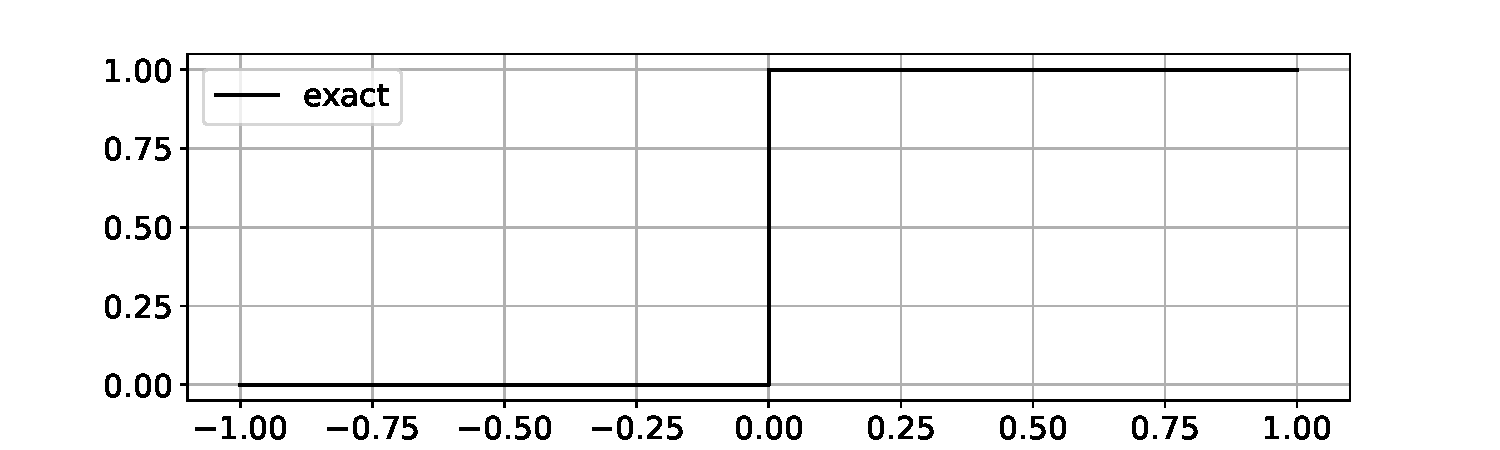
\includegraphics[width=0.8\textwidth]{Error_Funcion.pdf}
  \caption{$Error Function$ }
\end{figure}
\begin{figure}[!ht]

  \centering
  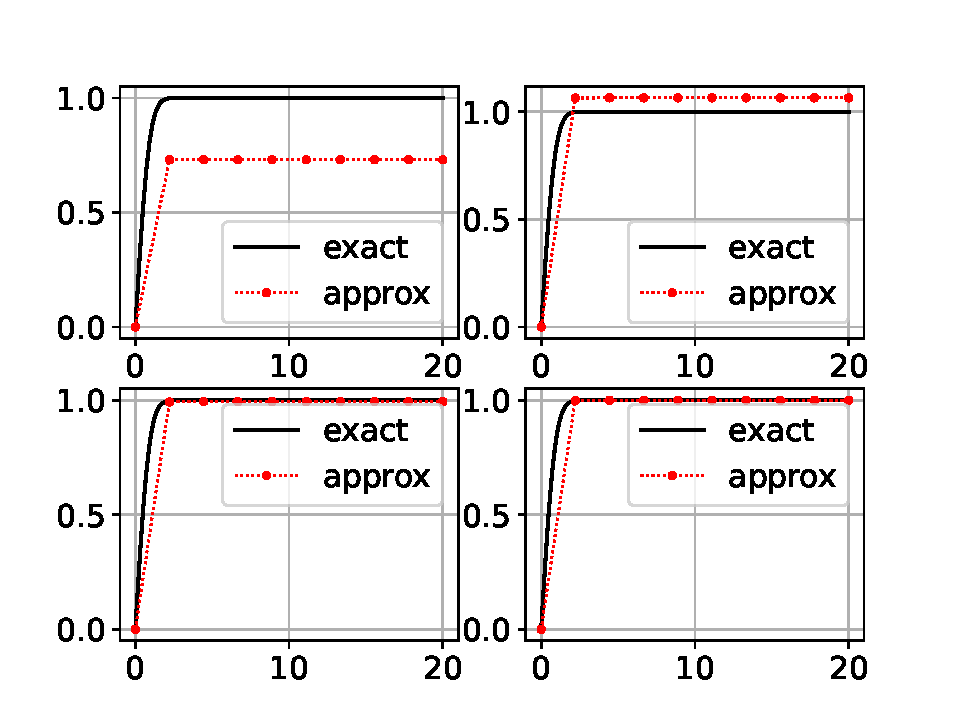
\includegraphics[width=0.8\textwidth]{Error_Funcion1.pdf}
  \caption{$Error Function\textunderscore for\textunderscore N = 1, 2, 3, 4$ }
\end{figure}

이처럼, 우리의 예상대로 N의 값이 커질 수록 더 abs error 값이 줄어들면서 실제 값과 유사하게 적분이 될 수 있음을 볼 수 있다.
\pagebreak












\section{Double Integral}
\subsection{Problem Recognition} 
\begin{equation}
I = \int_{1}^{2} \int_{0}^{1} y^x dx dy
\approx 1.2292741342880657562
\end{equation}

이번에는 함수 I를 구해야 하는데, $dx$와 $dy$에 대하여 각각의 범위에 대해 적분을 시켜주려고 한다. $Y(x)$ 를 적분하려면, 먼저 $dx$ 에 대하여 적분을 해준 뒤, $y$ 에 대하여 적분을 해주어야 한다.

\subsection{Development of a solution} 

먼저 우리는 x에 대한 식을 y의 변수와 함께 저장하는 함수를 지정해 주어야 한다. 즉, x값이 변하더라도 y값은 변하지 않는 함수를 만들고, 그 함수에서 $x$에 대하여 [0, 1] 의 범위를 적분해 준다. 그리고 다시 $y$에 대해 [1, 2] 범위를 적분해주면서 이차 적분을 풀어줄 수 있다.
 
 즉, 초기의 $F(x)$는 $x$에 대한 함수로 잡는다. 그리고 $x$에 대하여 적분을 하면 $F(y)$와 같으므로, 이를 다시 $y$에 대하여 적분을 한다. 이를 코드로 구현하면 다음과 같다.

\subsection{Execution and Assessment}
\begin{lstlisting}[language=Python]
def inner_sum(y):
    return min_fixed_any_range(lambda x: y**x, 0, 1, 11)
    
outer_sum = min_fixed_any_range(inner_sum, 1, 2, 11)

print("approximatio = {}, absolute error = {}"
      .format(outer_sum, abs(outer_sum - 1.2292741342880657562)))
     
approximatio = 1.229274134361613, absolute error = 7.354716835550335e-11
        \end{lstlisting}
실제 값과의 차를 구하면 0에 수렴할 정도로 작은 것을 볼 수 있다.  이것으로 SciPy 모듈의 fixed quad 모듈을 사용하지 않고, 직접 모듈을 만들어서 문제에 적용해 보았다.

\pagebreak
















\section{Orthogonality of Legendre polynomials}
\subsection{Problem Recognition} 
다음 Legendre 다항식의 직교성을 증명하여라.
\begin{equation}
\int_{-1}^1 P_m(x) P_n(x) dx = \frac{2}{2n + 1} \delta_{mn}
    \end{equation}

이 문제는 m 과 n이 임의의 정수일 때, [-1, 1]에서 Legendre 다항식 $P_m(x)$ 과 $P_n(x)$의 곱을 적분하였을 때, $m = n$이면 $\frac{2}{2n + 1}$, 다르면 $0$ 이 되는 것을 통하여, 다항식의 직교성을 증명하라는 문제이다. 이 문제를 풀기 위해서는 먼저, $P_m(x)$ 와  $P_n(x)$ 의 곱을 구하고, 그 값을 [-1, 1]에 대하여 적분을 시켜주면 된다. 이때, m, n은 임의의 정수이기 때문에, 같을 때와 다를 때를 나누어 확인해야 한다. 이는  $\delta_{mn}$ 의 특성을 유의해야 한다.

즉, 두가지 조건을 정리하면 다음과 같다.
\begin{itemize}
\item $n = m$ 인 경우,  $\int_{-1}^1 (P_n(x))^2 dx - \frac{2}{2n + 1}  = 0 $ 이 만족되어야 한다.
\item $n \neq m$인 경우, $\int_{-1}^1 P_m(x) P_n(x) dx = 0 $이 만족되어야 한다.
\end{itemize}

\subsection{First Condition} 
먼저 첫번째 조건이 성립하는지를 풀기 위해서, legendre(m) 을 이해하면, $m$에 어떠한 임의의 정수를 넣었을 때, 르장드르 다항식을 나타내는 함수이다. 유의해야 할 것은, legendre() 모듈은 함수를 나타내는 것이다. 따라서, 우리는 $F_m(x) = Legendre(m, x)$로 잡고, 원하는 문제를 풀 수 있다. 르장드르 모듈에서는 따로 x를 인자로 두지 않기 때문에, $F_m(x) = Legendre(m, x)$ 로 나타내지 않고, Legendre(m)으로 나타내면 된다. 이와 관련하여 몇가지 코드를 확인하면,
\begin{lstlisting}[language=Python]
import random
n, m = random.randint(0,10), random.randint(0,10)

def P_m(m): 
    return min_fixed_any_range(legendre(m), -1, 1, 10)
print(legendre(m) )

       4             3        2
4.375 x + 4.857e-16 x - 3.75 x + 2.429e-16 x + 0.375
        \end{lstlisting}
이렇게 위에서 언급했던 것 처럼, m에 임의의 정수를 넣으면 르장드르 다항식을 보여주는 함수이다. 이때, 르장드르 다항식은, m에 따라서 짝함수와 홀함수가 결정되는데, 위의 식에서는 $x^3$처럼 홀수 차수 항을 볼 수 있지만 계수는 0이므로 고려하지 않아도 된다. 이제 무작위의 $n$, $m$에 대해서 $n = m$ 이 성립할 때, 위의 조건에 만족하는지 확인할 것이다.

\begin{lstlisting}[language=Python]
import random
def P_m_P_M(m,n):
    return legendre(m) * legendre(n)
for i in range(10):
    n = random.randint(0,11)
    m = n
    print(f"n = {n}, m = {m}")
    print((2 / (2 * n + 1)) - min_fixed_any_range(P_m_P_M(m,n), -1, 1, 30))
    
n = 4, m = 4
-8.520961713998076e-15
n = 9, m = 9
-4.3921810632951974e-13
n = 10, m = 10
-4.626687921671646e-12
n = 6, m = 6
-1.6375789613221059e-15
n = 1, m = 1
-5.329070518200751e-15
n = 0, m = 0
0.0
n = 6, m = 6
-1.6375789613221059e-15
n = 9, m = 9
-4.3921810632951974e-13
n = 2, m = 2
-6.827871601444713e-15
n = 10, m = 10
-4.626687921671646e-12
        \end{lstlisting}
범위를 [0, 10] 으로 두고 계산하였지만, 만약, 범위가 10이상 커지게 되면 르장드르 다항식의 차수가 많아지게 되면서, 이를 적분하는데 많은 오차가 발생하게 된다. 따라서 이를 막으려면, 적분을 추산하는 함수의 N의 크기가 더욱 커져야 한다. 만약, 범위를 [10, 21] 로 두고, N = 5 인 경우,

\begin{lstlisting}[language=Python]
n = 14, m = 14
-6.884520453720455e-10
n = 21, m = 21
-0.00011664384684553081
n = 21, m = 21
-0.00011664384684553081
n = 18, m = 18
-4.849815616859987e-06
n = 21, m = 21
-0.00011664384684553081
n = 17, m = 17
7.57868260294059e-07
n = 10, m = 10
-4.626687921671646e-12
n = 15, m = 15
-4.713122087052213e-09
n = 15, m = 15
-4.713122087052213e-09
n = 21, m = 21
-0.00011664384684553081
\end{lstlisting}

이처럼, Legendre 다항식의 차수가 21에 가까워 질 수록, 오차 값이 커져버리는 경우가 발생할 수 있다. 따라서 적분 값을 추산할 때, N의 값을 조율하면서 맞추어 줄 수 있다. 정리하면, 우리가 적절하게 정한 오차 범위내에서 $n = m$ 을 가정하여 계산했을 경우, 우리가 초기에 설정한 첫번째 조건에 성립하는 것을 볼 수 있다. 그러면 두번째 조건이 타당한지를 확인해 볼 것이다.



\subsection{Second Condition}
두번째 조건은, $n \neq m$인 경우, $\int_{-1}^1 P_m(x) P_n(x) dx = 0 $이 만족되어야 한다. 이를 확인하기 위해선, 위에서 사용한 방식에서, n 과 m을 다르게 배치하므로써, 문제를 해결할 수 있다.

\begin{lstlisting}[language=Python]
import random

def P_m_P_M(m,n):
    return legendre(m) * legendre(n)

for i in range(10):
    n = random.randint(0,11)
    m = random.randint(1,12) - 1
    print(f"n = {n}, m = {m}")
    print(min_fixed_any_range(P_m_P_M(m,n), -1, 1, 30))
    
n = 2, m = 5
-2.0990154059319366e-16
n = 5, m = 8
1.215954420485943e-14
n = 3, m = 11
1.8747243341055153e-13
n = 6, m = 9
-2.9786936805997755e-14
n = 8, m = 6
2.3614790678472275e-14
n = 6, m = 0
8.934693263018545e-15
n = 6, m = 11
2.1583342751929635e-13
n = 4, m = 5
-8.795048023202412e-16
n = 8, m = 4
8.455042221910958e-15
n = 11, m = 5
1.5622919624647125e-13
    
    
\end{lstlisting}
이때 우리는 n, m을 서로 다른 정수로 표현하기 위해서 -1 을 취했는데, n과 m은 무작위 정수이므로 $n < m$ 이나 $n > m$ 에 대하여 고려할 필요가 없다. ($n = m,  m = n$을 대입하면 똑같다.) 따라서 이 결과값을 확인하면 모두 0에 수렴하기 때문에, 우리가 초기에 설정한 두번째 조건에도 만족하는 것을 볼 수 있다. 

\subsection{Execution and Assessment}
초기에 결정한 두가지 조건
\begin{itemize}
\item $n = m$ 인 경우,  $\int_{-1}^1 (P_n(x))^2 dx - \frac{2}{2n + 1}  = 0 $ 이 만족되어야 한다.
\item $n \neq m$인 경우, $\int_{-1}^1 P_m(x) P_n(x) dx = 0 $이 만족되어야 한다.
\end{itemize}
가 성립하므로 따라서 우리는

\begin{equation}
\int_{-1}^1 P_m(x) P_n(x) dx = \frac{2}{2n + 1} \delta_{mn}
    \end{equation}
이 성립함을 증명할 수 있고 따라서 두 르장드르 다항식은 직교성을 가진다는 것을 확인할 수 있다.









\pagebreak
\section{Orthogonality of Bessel funcions} 
\subsection{Problem Recognition} 
 이번에는 베셀 함수의 직교성을 증명하는 문제이다.
우리는 Bessel 함수에서  $\alpha$ 와 $\beta$가 $J_p$이 영점이라면, $\alpha$ 와 $\beta$가 같은 경우와 다른 경우의 값이 아래의 조건에 만족하는지 확인해 볼 것이다. 

\begin{equation}
\begin{split}
    \int_0^1 &J_p(\alpha x) J_p(\beta x) x dx
    \end{split}   
    = \frac{1}{2} (J_{p + 1})^2(\alpha) = \frac{1}{2} (J_{p - 1})^2(\alpha) = \frac{1}{2} (J_p')^2(\alpha)
   		  , \quad \quad\quad\alpha = \beta
        \end{equation}

\begin{equation}
\begin{split}
    \int_0^1 &J_p(\alpha x) J_p(\beta x) x dx
    \end{split}   
    =  0
   		  , \quad \quad\quad\alpha \neq \beta
        \end{equation}

유의해야 할 것은 바로, (12) 식에서 볼 수 있는데, $J_p'^2(\alpha)$ 값을 유추해야 한다. 이는 Sympy 의 Derivative() 모듈을 통해 도함수를 구할 수 있으나, 베셀함수의 특징을 생각하면, 어렵지 않게 유추할 수 있다. 바로, 베셀 함수의 반복 관계를 이용하면 된다. 베셀 함수의 반복 관계를 잠시 인용하면,

\begin{equation}
\begin{array}{c}

\displaystyle
\frac{d}{dx} (x^p J_p(x))
=
x^p J_{p - 1}(x)
\\

\displaystyle
\frac{d}{dx} (x^{-p} J_p(x))
=
-x^{-p} J_{p + 1}(x)
\\

\displaystyle
J_{p - 1}(x) + J_{p + 1}(x)
=
\frac{2p}{x} J_p(x)
\\

\displaystyle
J_{p - 1}(x) - J_{p + 1}(x)
=
2 J_p'(x)


\displaystyle
J_p'(x)
=
-\frac{p}{x} J_p(x) + J_{p - 1}(x)

\frac{p}{x} J_p(x) - J_{p + 1}(x)
\end{array}
        \end{equation}
        이 관계중에서 우리는 $J_{p - 1}(x) - J_{p + 1}(x)=2 J_p'(x)$ 을 이용하여 베셀 함수의 도함수를 구할 것이다.
        
\subsection{Development of a solution} 
이제, 앞서서 legendre 다항식의 직교성을 구한 것 처럼 두가지의 조건을 성립하는지 확인할 것이다. 조건은 다음과 같다.
\begin{itemize}

\item$ \alpha = \beta$의 경우, \\
$G(x) =  \int_0^1 J_p(\alpha x) J_p(\beta x) x dx - \frac{1}{2} (J_{p + 1})^2(\alpha) = 0  \\
H(x) =  \frac{1}{2} (J_{p - 1})^2(\alpha) - \frac{1}{2} (J_p')^2(\alpha) = 0 $.  을 만족해야 한다.




\item $\alpha \neq \beta$인 경우,  $I(x) = \int_0^1 J_p(\alpha x) J_p(\beta x) x dx = 0$. 을 만족되어야 한다.
\end{itemize}

베셀함수는 Scipy의 special.jn 모듈을 통하여 베셀 함수를 나타낼 수 있다. 하지만 유의할 것은, 위의 르장드르 방정식과 달리, x 값을 따로 설정해 주어야 한다. 또한, 베셀 함수의 해를 구해야 한다. 이는 Scipy.special 에서 jn\textunderscore zeros 모듈을 통해 구할 수 있다. 우리는 이 모듈을 통해 무작위의 $p$의 베셀 함수의 해를 구할 것이다. 이때,  jn\textunderscore zeros 에는 두가지 인수가 들어갈 수 있는데, jn\textunderscore zeros(n, N) 중에서 n은 베셀 함수의 차수 $p$이고, N은 해의 갯수를 나타낸다.

먼저 , n = [0, 10] 사이의 정수중에서 임의의 숫자 n을 만들고, 베셀 함수의 n차 식의 해 10개를 만들어, 변수 a, b에 random.choice() 를 통하여 저장한다. 변수 a, b는 베셀 함수의 $\alpha$ , $\beta$ 하는 값으로,  
 $special.jn(n, a*x)$ 와 $ special.jn(n, b*x)$ 함수의 적분값은 앞서 만든 min\textunderscore fixed\textunderscore any\textunderscore range를 통하여 두 베셀 함수의 곱의 [0, 1] 사이에서의 적분 값을 구해줄 것이다. 그리고 위 조건에서 $G(x)$ 와 $H(x)$  그리고 $I(x)$가 0이 되는지를 확인해 볼 것이다. 반복 횟수는 총 10번으로 하고, 무작위 10개의 n에 따라서 코드를 구현해보기로 한다. 


\begin{lstlisting}[language=Python]
import numpy as np
import matplotlib.pyplot as plt
plt.rcParams.update({'font.size': 15})
from scipy import optimize
from sympy import *
from scipy.special import jn_zeros 

x_zeros = []

#0~1 Solution
x_zeros = []
for i in range(10):
    n = random.randint(0,11)
    a = random.choice(jn_zeros(n, 10))
    b = random.choice(jn_zeros(n, 10))
    result = min_fixed_any_range(lambda x: x * special.jn(n, a * x) * special.jn(n, b * x) 
                    , 0, 1, 100)
    #j'p(a) used by Recursion Relations 
    third_hand = (special.jn(n - 1, a) - special.jn(n + 1, a)) / 2

    d1 = 1/2 * (special.jn(n + 1, a))**2 - (1/2 * (special.jn(n - 1, a))**2)# 1st hand - 2nd hand
    d2 = 1/2 * (special.jn(n + 1, a))**2 - (1/2 * (third_hand)**2) #2nd hand - 3rd hand
    
    if a == b:
        print(f"""a = b = {a},
        p = {n},
        G(x) = 1st hand - 2nd hand = {d1}, 
        H(x) = 2nd hand - 3rd hand = {d2}""")
        print('-'*50)
    else:
        print(f"""a = {a}, b = {b}, p = {n}, 
        I(x) = {result}""")
        print('-'*50)
        \end{lstlisting}

\subsection{Execution and Assessment}
\begin{lstlisting}[language=Python]
a = 19.61596690396692, b = 40.11182327095424, p = 11, 
I(x) = -1.0983110328872428e-17
--------------------------------------------------
a = 13.589290170541217, b = 20.320789213566506, p = 6, 
I(x)= -1.7686528310885834e-17
--------------------------------------------------
a = 19.615858510468243, b = 32.189679910974405, p = 1, 
I(x) = -2.0534590427073046e-17
--------------------------------------------------
a = b = 28.62661830729114,
p = 5,
G(x) = 1st hand - 2nd hand = 0.0, 
H(x) = 2nd hand - 3rd hand = 0.0
--------------------------------------------------
a = 28.62661830729114, b = 38.15986856196713, p = 5, 
I(x) = 1.3329975556429909e-17
--------------------------------------------------
a = b = 19.615858510468243,
p = 1,
G(x) = 1st hand - 2nd hand = -6.938893903907228e-18, 
H(x) = 2nd hand - 3rd hand = -6.938893903907228e-18
--------------------------------------------------
a = b = 13.015200721698434,
p = 3,
G(x) = 1st hand - 2nd hand = -7.979727989493313e-17, 
H(x) = 2nd hand - 3rd hand = -3.8163916471489756e-17
--------------------------------------------------
a = 7.015586669815619, b = 16.470630050877634, p = 1, 
I(x) = 1.0906488304388306e-17
--------------------------------------------------
a = 27.19908776598125, b = 24.01901952477111, p = 4, 
I(x) = 2.692116148956487e-17
--------------------------------------------------
a = 14.37253667161759, b = 24.01901952477111, p = 4, 
I(x) = 2.397629732142272e-17
\end{lstlisting}
 
위에서 구한 베셀 함수 조건 $G(x)$ 와, $H(x)$의 실행 결과는 다음과 같다.  조건문에 의하여, $\alpha$와  $\beta$값이 같으면, $G(x)$ 와 $H(x)$ 값이 0으로 나오고,  $\alpha$와  $\beta$값이 다르면 I(x) 값이 0으로 나오는 것을 확인할 수 있다. 따라서 위에서 말한 조건 두가지가 모두 성립하므로, $J_p$의 영점에 따라 직교성을 보인 다는 것을 증명하였다. 
\pagebreak























\section{Table of Gauss-Legendre Quadrature Coefficients}
\subsection{Problem Recognition} 
앞서서 구한 min\textunderscore fixed\textunderscore any\textunderscore range 함수는 SciPy function의 scipy.special.roots\textunderscore legendre를 통하여 구한 $x_i$와 $w_i$값을 이용하여 Gauss-Legendre 방식으로 [a, b]사이의 범위의 적분 값을 추산하였다. 그러면 이번에는 $x_i$와 $w_i$값을 Scipy function이 아닌, Root FInding에서 다룬 해를 추산하는 방식으로 계산하여 값을 구해보도록 할 것이다. 문제를 접근하기전 조건은 다음과 같다.

\begin{itemize}
\item Legendre 다항식은 scipy.special.legendre를 통하여 사용할 수 있다.
\item $P_n$에서 [-1, 1]에서 0을 만족하는 해를 찾을때, scipy.optimize.root\textunderscore scalar 또는 앞서서 다룬 Root Finding의 예제 코드를 이용할 수 있다
\item 
\begin{itemize}
\item 근에는 0이 포함되어야 한다.
\item 근은 y축에 대하여 대칭을 이룬다
\item 근은 n에 대하여 [-1, 1]을 bracket으로 두어, $\{-1, \dots, x_i^{(n-1)}, \dots, 1\}$ 범위내에서
$x_1^{(n)} \in (-1, x_1^{(n-1)})$와 $x_2^{(n)} \in (x_1^{(n-1)}, x_2^{(n-1)})$를 만족해야 한다.

\end{itemize}
\item Weights는 다음의 공식을 이용하여라. \\$w_i = \frac{2(1 - x_i^2)}{n^2 P_{n - 1}^2(x_i)}$
\end{itemize}
위에서 구한 근을 scipy.special.roots\textunderscore legendre와 비교하여 계산값을 확인해 보자.
먼저 근을 구하기 위해, optimize.root\textunderscore scalar를 사용하여 근을 계산할 것이다. bracket을 정했기 때문에, bisection 방법과 secant 방법 등을 이용할 수 있지만, 이때 bisection의 경우, 함수가 [-1, 1] 범위 내에서 경계의 값 두 개의 부호가 같을 경우 사용할 수 없기 때문에, secant 방법을 사용한다. 

\subsection{Development of a solution} 
\begin{lstlisting}[language=Python]
import random

def frank(n, x):
    leg = legendre(n)
    p_n = leg(x)
    return p_n


def N(n):
    N = n
    partition = np.linspace(-1, 1, 10 * n)
    sollist = []
    sollist_1 = []
    a = []
    wlist = []

    for (l, r) in zip(partition[:-1], partition[1:]):
        sol = optimize.root_scalar(legendre(N), x0 = l, x1 = r,
                                  method = 'secant')
                           
        sollist.append(abs(round(sol.root, 7)))
    
    sollist_1 = [i for i in sollist if abs(i) > 10e-5 and abs(i) < 1 and abs(i) > 0.0617]

    for i in range(len(sollist_1)):
        for j in sollist_1:
            if j - sollist[i] < 0.01 and  j * sollist[i] > (sollist[i])**2:
                if j == sollist[i]:
                    continue
                sollist_1.remove(j)

    a = list(set(sollist_1))
    a2 = []
    if N % 2 != 0:
        a.append(0)

    for x in a:
        if x != 0:
            a2.append(-1 * x)

    b = a + a2
    for x in b:
        w = (2 * (1 - x**2)) / (N**2 * frank(N-1, x)**2)
        wlist.append(w)



    
    return(b, wlist , len(b))
 \end{lstlisting}
 
    
    
 \subsection{Execution and Assessment}
 \begin{lstlisting}[language=Python]
 N(1)
 ([0], [2.0], 1)
 
 N(2)
 ([0.5773503, -0.5773503], [0.9999998399046123, 0.9999998399046123], 2)
 
 N(3)
([0.7745967, 0, -0.7745967],
 [0.5555552908284657, 0.8888888888888885, 0.5555552908284658],
 3)
 
 N(11)
 ([0.8870626,
  0.730152,
  0.2695432,
  0.5190961,
  0.1375864,
  0,
  -0.8870626,
  -0.730152,
  -0.2695432,
  -0.5190961,
  -0.1375864],
 [0.12558036655571,
  0.1862902499023628,
  0.2628044637583425,
  0.2331938807413568,
  18.53831023130149,
  0.2729250867779006,
  0.1255803665557089,
  0.186290249902364,
  0.26280446375834254,
  0.23319388074135666,
  18.53831023130156],
 11)
 
 N(20)
 ([0.9122344,
  0.839117,
  0.6360537,
  0.7463319,
  0.4436109,
  0.510867,
  0.3737061,
  0.2277859,
  0.0765265,
  -0.9122344,
  -0.839117,
  -0.6360537,
  -0.7463319,
  -0.4436109,
  -0.510867,
  -0.3737061,
  -0.2277859,
  -0.0765265],
 [0.06267245254242511,
  0.08327646207685989,
  0.11819442975809738,
  0.10193016641167287,
  0.5619873869287483,
  0.13168864590801288,
  0.14209608006508162,
  0.1491729129292063,
  0.15275339756771986,
  0.06267245254242489,
  0.08327646207686057,
  0.118194429758097,
  0.10193016641167345,
  0.5619873869287483,
  0.13168864590801257,
  0.14209608006508156,
  0.14917291292920637,
  0.1527533975677196],
 18)
\end{lstlisting}
 







\end{document}